\documentclass[fyp]{socreport}
\usepackage{fullpage}
\usepackage{hyperref}
\usepackage{amsmath}
\usepackage{apacite}
\usepackage{booktabs}
\usepackage{graphicx}
\begin{document}
\pagenumbering{roman}
\projyear{2019/20}
\projnumber{H226080}
\author{Kuan Sheng Yuan, Jethro}
\title{Spiking Neural Networks}
\advisor{Dr.\ Harold Soh}
\deliverables{
	\item Report: 1 Volume}
\maketitle

\begin{abstract}
  Spiking neural networks are third-generation neural networks that are well
  positioned to supersede the state-of-the-art deep learning methods in problems
  that are temporal in nature. Difficulties in training spiking neural networks
  mean they see little use outside of academic research. We evaluate a
  state-of-the-art gradient-based spiking neural network architectures, and
  propose its application in two settings: (1) as an agent in a reinforcement
  learning environment, and (2) as a controller in a robotics setting. We train
  spiking neural agents on the OpenAI gym environment, as well as a classifier
  on a novel multi-modal event-based dataset. The spiking neural network agents
  outperform artificial neural networks with fewer parameters, and a desirable
  property of being able to make early predictions.

  \begin{keywords}
    Spiking Neural Networks, Reinforcement Learning, Multi-modal Machine Learning
  \end{keywords}

  \begin{implement} Python 3, PyTorch
  \end{implement}
\end{abstract}

% \listoffigures
% \listoftables
\tableofcontents

\chapter{Introduction}

\section{Motivation}

Deep neural networks (DNNs) have seen widespread industrial adoption, across
tasks such as machine translation, image recognition, and in recommender
systems. The remarkable success of deep learning can be attributed to
advancements in gradient-based training methods and model architectures,
allowing larger and deeper models to be trained and deployed.

Spiking Neural Networks (SNNs) is a nascent area of study. SNNs use neuronal
units called spiking neurons which closely mimic the biological neuron,
communicating via sparse, discrete spikes. This allows SNNs deployed on
neuromorphic hardware to achieve favorable properties such as low power
consumption, and fast inference. SNNs are rarely seen outside of academic
research, because they remain difficult to train and have yet to outperform
DNNs.

This thesis is a study of spiking neural networks and their applications. We are
motivated by recent advancements in gradient-based training methods for spiking
neural
networks~\cite{NIPS2018_7415,NIPS2018_7417,neftci19_surrog_gradien_learn_spikin_neural_networ},
which has brought about a resurgence of interest in the field.

\section{Research Outline}

In \autoref{chp:background}, we first provide a comprehensive study on SNNs.

The central property of SNNs that we exploit is the following:

\begin{quote}
  Unlike DNNs, SNNs are temporal in nature: spiking neurons store as state their
  membrane potential, which changes over time.
\end{quote}

This property of SNNs positions them to supersede state-of-the-art DNNs in
problems that are temporal in nature.

In \autoref{cha:snnrl}, we evaluate the feasibility of spiking neural networks
as agents in a reinforcement learning setting. Reinforcement learning episodes
often have a temporal element, due to the interdependence between states and
actions in the environment. We hypothesised that spiking neural agents are well
suited in many reinforcement learning settings.

In \autoref{cha:vtsnn}, we contribute an event-driven visual-tactile
spiking-neural network (VT-SNN), which enables fast perception on two
event-based sensors: the NeuTouch~\cite{aiskinLee}, and the Prophesee event
camera. This is a joint project between our group, the Collaborative Learning \&
Adaptive Robots (CLeAR) group, and the AiSKIN research group, which contributed
the NeuTouch neuromorphic touch sensor. Spiking neural networks are able to
naturally handle the sparse and discrete event-based data.

\chapter{Background\label{chp:background}}

This chapter provides background knowledge about spiking neural networks. It
reviews the differences between deep neural networks, and spiking neural
networks (\ref{sec:gener-neur-netw}). It introduces the basics of spiking neural
networks (\ref{sec:spiking-neuron-model}), and its benefits
(\ref{sec:motiv-spik-neur}). Finally, we discuss how to train spiking neural
networks (\ref{sec:train-spik-neur}), and give some future directions.

\section{The Generations of Neural Networks\label{sec:gener-neur-netw}}

Neural network models can be classified into three generations, according to
their computational units: perceptrons, non-linear units, and spiking
neurons~\cite{MAASS19971659}.

Perceptrons can be composed to produce a variety of models, including Boltzmann
machines and Hopfield networks. Non-linear units are currently the most widely
used computational unit, responsible for the explosion of progress in machine
learning research, in particular, the success of deep learning. These units
traditionally apply differentiable, non-linear activation functions such across
a weighted sum of input values.

There are two reasons second-generation computational units have seen so much
success. First, the computational power of these units is greater than that of
first-generation neural networks. Networks built with second-generation
computational units with one hidden layer are universal approximators for any
continuous function with a compact domain and range~\cite{Cybenko1989}. Second,
networks built with these units are trainable with well-researched
gradient-based methods, such as backpropagation.

The third generation of neural networks use computational units called spiking
neurons. Much like our biological neurons, spiking neurons are connected to each
other at synapses, receiving incoming signals at the dendrites and sending
spikes to other neurons via the axon. Each computational unit stores some state:
in particular, it stores its membrane potential at any point in time. Rather
than fire at each propagation cycle, these computational units fire only when
their individual membrane potentials crosses its firing threshold. A simple
spiking neuron model is given in \autoref{spike_model}.

From this section onwards, we shall term second-generation neural networks
Artificial Neural Networks (ANNs), and third-generation neural networks Spiking
Neural Networks (SNNs).

\section{A Spiking Neuron Model\label{sec:spiking-neuron-model}}

In spiking neural networks, neurons exchange information via spikes, and the
information received depends on:

\begin{description}
\item[{Firing frequencies}] The relative timing of pre and post-synaptic spikes,
and neuronal firing patterns
\item[{Identity of synapses used}] Which neurons are connected, whether their
synapses are inhibitory or excitatory, and synaptic strength
\end{description}

Each neuron has a corresponding model that encapsulates its state: the current
membrane potential. As with the mammalian brain, incoming spikes increase the
value of membrane potential. The membrane potential eventually decays to resting
potential in the absence of spikes. These dynamics are often captured via
first-order differential equations. Here we define the Spike Response Model
(SRM), a simple but widely-used model describing the momentary value of a neuron
\(i\).

We define for presynaptic neuron \(j\),
\(\epsilon_{ij}(t) = u_{i}(t) - u_{\text{rest}}\). For a few input spikes, the
membrane potential responds roughly linearly to the input spikes:

\begin{equation} u_i{t} = \sum_{j}\sum_{f} \epsilon_{ij}(t - t_j^{(f)}) + u_{\text{rest}}
\end{equation}

SRM describes the membrane potential of neuron \(i\) as:

\begin{equation} u_i{t} = \eta (t - \hat{t_i}) + \sum_{j}\sum_{f} \epsilon_{ij}(t - t_j^{(f)}) + u_{\text{rest}}
\end{equation}

where \(\hat{t_i}\) is the last firing time of neuron \(i\).

We refer to moment when a given neuron emits an action potential as the firing
time of that neuron. We denote the firing times of neuron \(i\) by \(t_i^{(f)}\)
where \(f = 1,2,\dots\) is the label of the spike.  Then we formally denote the
spike train of a neuron \(i\) as the sequence of firing times:

\begin{equation} S_i(t) = \sum_{f} \delta\left( t - t_i^{(f)} \right)
\end{equation}

where \(\delta(x)\) is the Dirac-delta function with \(\delta(x) = 0\) for
\(x \ne 0\) and \(\int_{-\infty}^{\infty} \delta(x)dx = 1\). Spikes are thus
reduced to points in time.

\section{Motivating Spiking Neural Networks\label{sec:motiv-spik-neur}}

Since second-generation neural networks have excellent performance, why bother
with spiking neural networks? In this section, we motivate spiking neural
networks from various perspectives.

\subsection{Information Encoding}

To directly compare ANNs and SNNs, one can consider the real-valued outputs of
ANNs to be the firing rate of a spiking neuron in steady state. In fact, such
rate coding has been used to explain computational processes in the
brain~\cite{pfeiffer2018deep}. Spiking neuron models encode information beyond
the average firing rate: these models also utilize the relative timing between
spikes~\cite{guetig14_to_spike_or_when_to_spike}, or spike phases (in-phase or
out-of-phase). These time-dependent codes are termed temporal codes, and play an
important role in biology. First, research has shown that different actions are
taken based on single spikes~\cite{stemmler96_singl_spike_suffic}. Second,
relying on the average firing rate would greatly increase the latency of the
brain, and our brain often requires decision-making long before several spikes
are accumulated.  It has also been successfully demonstrated that temporal
coding achieves competitive empirical performance on classification tasks for
both generated datasets, as well as image datasets like MNIST and
CIFAR~\cite{comsa19_tempor_codin_spikin_neural_networ}.

\subsection{Biological Plausibility\label{bioplausible}}

A faction of the machine learning and neurobiology community strives for
emulation of the biological brain. There are several incompatibilities between
ANNs and the current state of neurobiology that are not easily reconciliated.

First, neurons in ANNs communicate via continuous-valued activations.  This is
contrary to neurobiological research, which shows that communication between
biological neurons communicate by broadcasting spike trains: trains of action
potentials to downstream neurons. The spikes are to a first-order approximation
of uniform amplitude, unlike the continuous-valued activations of ANNs.

Second, backpropagation as a learning procedure also presents incompatibilities
with the biological brain~\cite{TAVANAEI201947}.  Consider the chain rule in
backpropagation:

\begin{equation} \label{chainrule} \delta_{j}^{\mu}=g^{\prime}\left(a_{j}^{\mu}\right) \sum_{k} w_{k j} \delta_{k}^{\mu}
\end{equation}

\(\delta_{j}^{\mu}\) and \(\delta_{k}^{\mu}\) denote the partial derivatives of
the cost function for input pattern \(\mu\) with respect to the net input to
some arbitrary unit \(j\) or \(k\). Unit \(j\) projects feed-forward connections
to the set of units indexed by \(k\).  \(g(\cdot)\) is the activation function
applied to the net input of unit \(j\), denoted \(a_j^{\mu}\), \(w_{kj}\) are
the feedforward weights projecting from unit \(j\) to the set of units indexed
by \(k\).

The chain rule formulation presents two problems. First, the gradients
\(g'(\cdot)\) requires derivatives, but \(g(\cdot)\) in spiking neurons is
represented by sum of Dirac delta functions, for which derivatives do not
exist. Second, the expression \(\sum_{k} w_{k j} \delta_{k}^{\mu}\) uses
feedforward weights in a feedback fashion. This mean that backpropagation is
only possible in the presence of symmetric feedback weights, but these do not
exist in the brain. In addition, during backpropagation the error assignment for
each neuron is computed using non-local information.

\subsection{Neuromorphic Hardware\label{neuromorphic}}

In a traditional Von Neumann architecture, the logic core operates on data
fetched sequentially from memory. In contrast, in neuromorphic chips both
computation and memory are distributed across computational units that are
connected via synapses. The neuronal architecture and parameters hence play a
key role in information representation and define the computations that are
performed.

It has also been observed that spike-trains in the mammalian brain are often
sparse in time, suggesting that timing and relative timings of spikes encode
large amounts of information. Neuromorphic chips implement this same sparse,
low-precision communication protocol between neurons on the chip, and by
offering the same asynchronous, event-based parallelism paradigm that the brain
uses, are able to perform certain workloads with much less power than Von
Neumann chips.

These integrated circuits are typically programmed with spiking neural
networks. Examples of such chips include IBM's TrueNorth~\cite{Merolla668} and
Intel's Loihi~\cite{davies2018loihi}. Because spiking neural networks have not
yet been successfully trained on many tasks, neuromorphic chips has seen little
practical use. These chips have only recently been successfully used in robotic
navigation~\cite{SnnSlam}, and solving graph problems by manual construction of
the network graph~\cite{Severa2016SpikingNA}.

\section{Training Spiking Neural Networks\label{sec:train-spik-neur}}

As explained in \autoref{neuromorphic}, it is desirable to train spiking neural
networks to perform arbitrary tasks, utilizing power-efficient neuromorphic
chips that break the Von Neumann bottleneck. We classify the training strategies
by their usage of gradients, and discuss certain optimization techniques.

\subsection{Non-gradient based methods}

Spiking neurons communicate via spikes, hence, unlike ANNs, gradients are
non-existent. In addition, backpropagation is not biologically plausible (see
\autoref{bioplausible}). This motivates the use of plasticity-based methods and
evolutionary strategies for training SNNs.

One category of learning rules used in SNNs are local learning rules.  These
rules include Hebbian learning (neurons that fire together wire together), and
its extension: the spike-timing-dependent-plasticity rule (STDP). Inspired by
experiments in neuroscience, central to these learning rules is the theme that
neuron spike ordering and their relative timings encode information. STDP
adjusts the strength of connections between neurons using the relative timing of
a neuron's output and its input potentials (hence, spike-timing dependent).

In machine learning terminology, the weights of the synapses are adjusted
according to fixed rules for each training example. Each synapse is given a
weight \(0 \le w \le w_{\max}\), characterizing its strength, and its change
depends on the exact moments \(t_{pre}\) of pre-synaptic spikes and \(t_{post}\)
of post-synaptic spikes~\cite{sboev18_spikin_neural_networ_reinf_learn}:

\begin{equation} \Delta w=\left\{\begin{array}{l}{-\alpha \lambda \cdot \exp \left(-\frac{t_{\mathrm{pre}}-t_{\mathrm{post}}}{\tau_{-}}\right), \text {if } t_{\mathrm{pre}}-t_{\mathrm{post}}>0} \\ {\lambda \cdot \exp \left(-\frac{t_{\mathrm{post}}-t_{\mathrm{pre}}}{\tau_{+}}\right), \text {if } t_{\mathrm{pre}}-t_{\mathrm{post}}<0}\end{array}\right.
\end{equation}

where \(\tau_{+}\) and \(\tau_{-}\) are time constants. \(\tau_{+} = 16.8ms\)
and \(\tau_{-} = 33.7ms\) are reasonable approximations obtained experimentally.

There are several libraries like BindsNET~\cite{10.3389/fninf.2018.00089} that
simulate SNNs on Von Neumann computers implementing these rules. Recent attempts
have been made to combine Reinforcement Learning and STDP:\@ both in solving RL
problems~\cite{10.3389/fninf.2018.00089}, and using the reinforcement learning
framework to train
SNN~\cite{10.3389/fnbot.2019.00018,10.3389/fnins.2018.00435}. However, SNNs
trained using the STDP learning rule have yet to achieve comparable performance
compared to ANNs on relatively simple datasets like MNIST~\cite{TAVANAEI201947}.

\subsection{Gradient-based methods}

Performance is important for practical applications, and gradient-based training
methods such as backpropagation has shown competitive performance. It is thus
desirable to train spiking neural networks with these gradient-based methods.

There are several problems with spike-compatible gradient-based methods. First,
most of these methods cannot train neurons in the hidden layers: they can only
train neurons at the final layer, that receive the desired target output
pattern~\cite{urbanczik09_gradien_learn_rule_tempot,training_deep_snn_bpp_lee}.
Second, the discontinuous, binary nature of spiking output needs to be
addressed. For example, SpikeProp approximates the membrane threshold function
at a local area with a linear function, introducing gradients and computing the
exact formulae for error backpropagation for synaptic weights and spike
times~\cite{spikeprop}. Others have modified the threshold function with a gate
function~\cite{NIPS2018_7417}, used the alpha transfer function to derive
gradient update rules~\cite{comsa19_tempor_codin_spikin_neural_networ}, and
approximate the dirac-delta spikes with a probability density
function~\cite{NIPS2018_7415}.

Another approach is converting trained ANN models into
SNNs~\cite{rueckauer16_theor_tools_conver_analog_to}. Common ANN layers such as
softmax, batch normalization and max-pooling layers have their corresponding
spiking counterparts.

Equilibrium Propagation was recently proposed to solve the neurobiological
incompatibilities of backpropagation~\cite{10.3389/fncom.2017.00024}. Because
the gradients are defined only in terms of local perturbations, the synaptic
updates correspond to the standard form of STDP.\@ The propagated signal encodes
the gradients of a well-defined objective function on energy-based models, where
the goal is to minimize the energy of the model. To resolve the issue of
communication using binary-valued signals, step-size annealing was used to train
spiking neural networks with Equilibrium Propagation
~\cite{pmlr-v89-o-connor19a}.

\subsection{Future Research Areas\label{sec:future-rese-areas}}

A nascent area is local learning on neuromorphic chips. Thus far spiking neural
networks are simulated and trained before deployment on a neuromorphic chip. In
Intel's Loihi chip, each core contains a learning engine that can update
synaptic weights using the 4-bit microcode-programmed learning rules that are
associated with that synapse. This opens up areas for online learning.

\chapter{Reinforcement learning in Spiking Neural Networks\label{cha:snnrl}}

To achieve the first milestone (see \autoref{sec:milestones}), I begin this
research project by conducting a survey on SNN architectures that use gradients
and have code readily available. We have found 2 repositories:

\begin{enumerate}
\item
\href{https://github.com/google/ihmehimmeli}{ihmehimmeli}~\cite{comsa19_tempor_codin_spikin_neural_networ}
\item
\href{https://github.com/bamsumit/slayerPytorch/}{SLAYER}~\cite{NIPS2018_7415}
\end{enumerate}

We establish baselines, and evaluate these models on the STMNIST dataset.

It must be noted that the small number of samples in this dataset results in
large error bars for each of the experiments conducted, and more samples must be
collected before any conclusions are statistically significant. My experiments
were run before the STMNIST dataset was updated. I have included my experimental
results on this small dataset, as well as experimental results attained
independently on the larger dataset for posterity.

\section{Milestone 1: Supervised Learning on the STMNIST dataset}

\subsection{The STMNIST dataset}

The STMNIST dataset is an unreleased dataset consisting of 200 samples, prepared
by handwriting digits from 0 to 9, on a $10 \times 10$ tactile sensor grid
\footnote{The STMNIST dataset preparation is a work-in-progress, and has grown
  to a sizable 7000 samples since I last worked with it.}. The data is of
dimension \((10, 10, t)\), where \(t\) is the number of time-steps for that
particular sequence, \(t\) goes up to \(20,000\). The values are either 0, -1 or
1, repesenting no spike, positive and negative spikes respectively. This dataset
poses a few unique challenges:

\begin{enumerate}
\item Unlike existing spiking datasets like the NMNIST
dataset~\cite{10.3389/fnins.2015.00481}, the data is highly sparse: at each
time-step, few neurons spike, which is consistent with spike trains that occur
in the brain.
\item The dataset has an extremely large number of time-steps, which is a
challenge for gradient-based methods such as backpropagation through time.
\end{enumerate}

This dataset is designed for the supervised learning task of predicting the
correct digit, given the spiking input.

\subsection{Establishing Baselines}

If we squash all time-steps together and binarize the values to 0s and 1s, we
re-obtain the hand-drawn digit\footnote{Colab notebook
\href{https://colab.research.google.com/drive/1EEZSOmGzvNcsGbCXiw1p7GyM5RBVv4uy}{here}.}. We
can then train a MLP or CNN on the resultant image with regular supervised
learning techniques. We use these trained models as our baselines. If it is
indeed true that relative spike timings encode useful temporal information, then
these baseline models discard all such temporal information, and should have
weaker performance.

This method achieves a test accuracy of about 75\%\footnote{Colab notebook
  \href{https://colab.research.google.com/drive/1Tig07aWvKKDnJ1VUwUf31wLpUjvupGDp}{here}.}. The
AiSKIN team has independently trained a CNN on the updated, larger dataset, and
obtained an accuracy of just above 80\%.

\subsection{Evaluating Ihmehimmeli}

We encode the information temporally as described in the paper, by using the
time to first spike for each cell in the 10 by 10 grid
~\cite{comsa19_tempor_codin_spikin_neural_networ}\footnote{Colab notebook
\href{https://colab.research.google.com/drive/144bSlbCXV8Rce0mAvq42byq3alMW7PXl}{here}.}. We
evaluate their model with the same hyperparameters the authors used for the
original MNIST problem, and achieved a similar accuracy of 75\%, demonstrating
that time-to-first-spike provides sufficient information for this classification
task.

\subsection{Evaluating SLAYER}

Because we had decided that the STMNIST dataset was not able to provide
conclusive results because of the small number of samples, we had given feedback
to the AiSKIN team to collect more data, and opted not to run this experiment
for SLAYER.\@ I had shifted my research focus towards the reinforcement learning
side of things after this decision.

SLAYER was eventually evaluated by other researchers in the lab group on the
larger dataset, with reported test accuracies of 92.7\%. This is significantly
higher than the baseline CNN model trained by the AiSKIN team.

I summarise the evaluation results in \autoref{tab:stmnist_results}.

\begin{table}[htbp]
\caption{\label{tab:stmnist_results} Test accuracies of models trained on the
STMNIST dataset. Caveat: the results have no error-bars, communicated via
word-of-mouth, and hyperparameters are not communicated. The objective of these
runs are to get a rough idea of whether these models are performant: this is not
the main evaluation task.}  \centering
\begin{tabular}{llll}
  \toprule
  Dataset & Baseline CNN & ihmehimmeli & SLAYER \\
  \midrule Initial & 75\% & 75\% & --- \\
  Updated & 80\% & --- & 92.7\%\\
  \bottomrule
\end{tabular}
\end{table}


\section{Milestone 2: Reinforcement Learning on the Cartpole Environment}

\subsection{The Cartpole Environment}


We use the Cartpole-v0 environment, a popular environment provided by
OpenAI.\@ The official description is as follows~\cite{openai_gym}:

\begin{quote} A pole is attached by an un-actuated joint to a cart, which moves
along a frictionless track. The system is controlled by applying a force of +1
or -1 to the cart. The pendulum starts upright, and the goal is to prevent it
from falling over. A reward of +1 is provided for every time-step that the pole
remains upright. The episode ends when the pole is more than 15 degrees from
vertical, or the cart moves more than 2.4 units from the center.

CartPole-v0 defines ``solving'' as getting average reward of 195.0 over 100
consecutive trials.
\end{quote}

\begin{figure}[htbp] \centering
  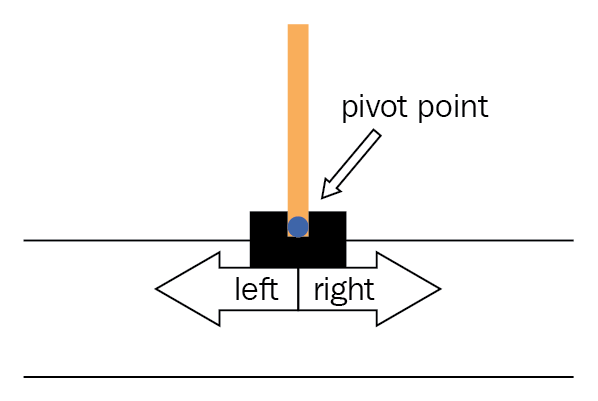
\includegraphics[width=.9\linewidth]{images/openai_gym.png}
  \caption{The OpenAI CartPole environment}
\end{figure}

\subsection{Training a Simple ANN agent}

First, we attempt to solve the problem with a simple MLP ANN agent that takes in
the four observations, and outputs as logits the probability of each action. The
action is then sampled from a 2-outcome categorical distribution with the logits
as the outcome probabilities. We do this so we can compare the performance of
the policies, learnt under the same conditions (learning rule, environment
parameters etc.).

Since SLAYER uses PyTorch, we implement vanilla policy gradients in PyTorch to
train the MLP agent. We use Sacred~\cite{klaus_greff-proc-scipy-2017} to log and
ensure reproducibility of our experiments.\footnote{This repository is hosted on
Github at \url{https://github.com/jethrokuan/snnrl/}. The repository is private,
request access as required.}

Experiments show that the ANN model learns to solve the environment quickly when
trained with VPG, as shown in \autoref{fig:vpg_mlp}. The agent obtains an
average episodic return of 200, ``solving'' the environment at 2000 time-steps.

\begin{figure}[htbp] \centering
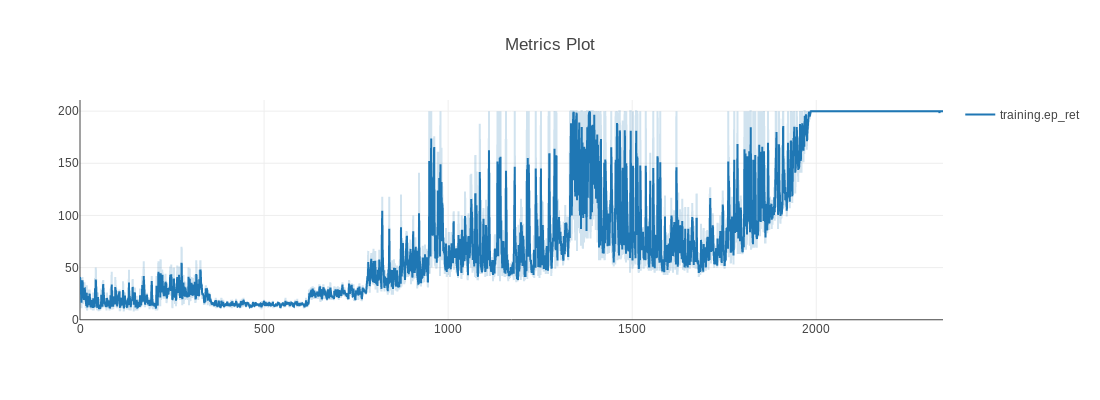
\includegraphics[width=.9\linewidth]{images/vpg_mlp.png}
\caption{\label{fig:vpg_mlp} Plot of average episode returns over time-steps for
a simple MLP agent.}
\end{figure}

\subsection{Training a SNN agent}

Similarly, we attempt to train the SLAYER model to solve the CartPole-v0. Each
SLAYER layer takes in a spike train as input and produces a spike train as
output. The objective function for supervised learning tasks such as
classification is defined in the paper, and is similar to
cross-entropy~\cite{NIPS2018_7415}.

Since the input to the Slayer model are spike trains, we require an encoder
mapping the environment observations into the fixed-length spike trains that
SLAYER accepts,as shown in \autoref{fig:slayer_rl}.

\begin{figure}[htbp] \centering
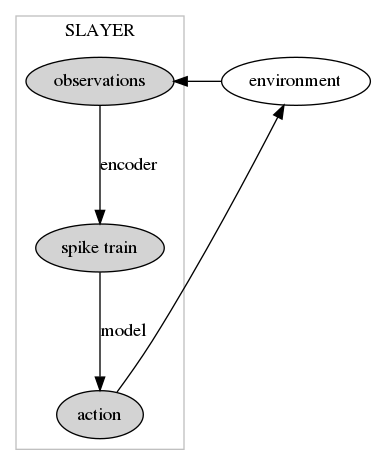
\includegraphics[height=7cm]{images/snn_encode.png}
\caption{\label{fig:slayer_rl} The SLAYER model requires an additional encoder
to transform the observations into spike trains as input.}
\end{figure}

We encode the observations by modelling the observations as Poisson
processes~\cite{heeger2000poisson}. First, we convert each of the four
observations into 2 non-negative observations: their absolute value, and their
sign. A negative value has an observation value of 0, and a positive value has
observation value of 1. We divide time into short, discrete intervals
\(\delta t\), and generate a sequence of random numbers \(x[i]\) uniformly
between 0 and 1. For each interval, if \(x[i] \le r \delta t\), generate a
spike. We produce spike trains of 300 time-steps as input to the SLAYER model
from the 8 observation values (scaled appropriately).

As shown in \autoref{fig:snn_vpg}, the SLAYER model fails to learn to solve the
problem.

\begin{figure}[htbp] \centering
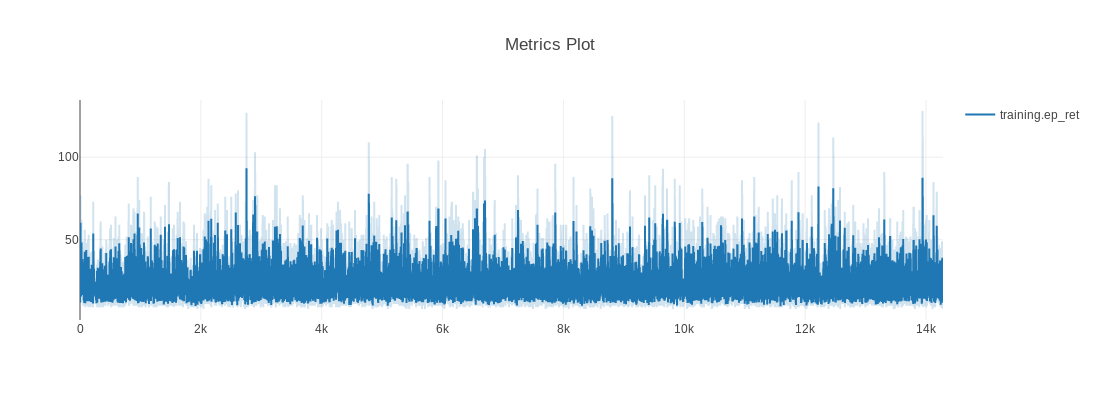
\includegraphics[width=.9\linewidth]{images/slayer_poisson.png}
\caption{\label{fig:snn_vpg} The SLAYER model with a Poisson encoder for the
observations fails to learn to solve the problem.}
\end{figure}

The problem likely resides in way encoding is done. The domain of the value of
some observations in the Cartpole environment is the range over all real
numbers, and encoding values over the entire range of real numbers is
tricky. There is no linear mapping, and changes in observation values may not
result in changes of noticeable magnitude in the mapped value.

There has, however, been works on encoding images into spike trains.  This is
particularly common as many spiking neural architectures are evaluated on a
converted MNIST image dataset. Hence, we move towards training spiking neural
networks on image observations.

\subsection{The ImageCartpole Environment}

To bypass the encoding issue described earlier, we turn towards training agents
on the pixels of the environment. We create a Cartpole environment such that the
observation is the difference in pixels of the current frame and the previous
frame. We term this modified environment ImageCartpole.

We train a simple CNN on this environment, using VPG.\@ Training this agent takes
significantly more time, as seen in \autoref{fig:imagecartpole_cnn}. However,
the agent is still able to learn from the observations, suggesting that this
environment is solvable by a SNN agent.

\begin{figure}[htbp] \centering
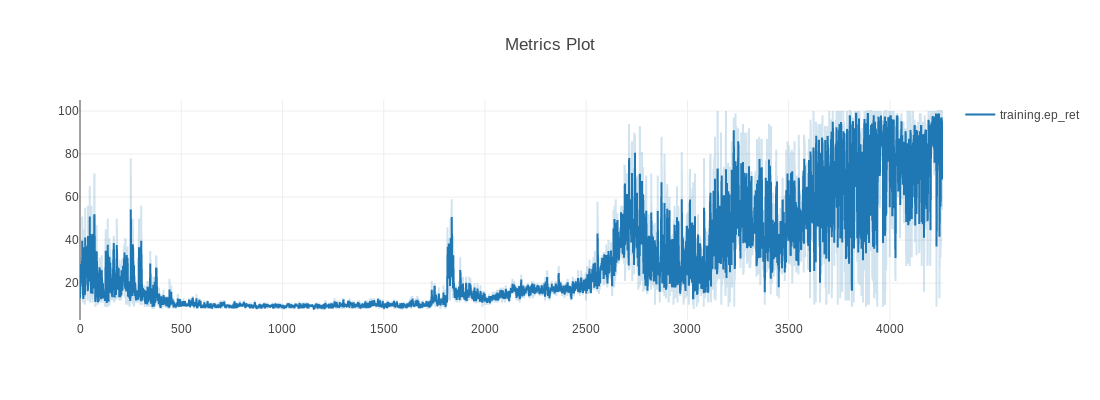
\includegraphics[width=.9\linewidth]{images/imagecartpole_cnn.png}
\caption{\label{fig:imagecartpole_cnn} Plot of the average episode return of a
CNN agent on the ImageCartpole environment over time.}
\end{figure}

At the time of submission, the SNN agent is unable to learn a good policy, but
more engineering work is required before any conclusions can be made.

\section{Future Work}

It is hoped that the SLAYER model is able to learn to solve simple environments
such as the Cartpole environment. Once it is established that gradient-based RL
methods also work for training SLAYER, we would move on towards milestones 3 and
4. If we are unable to learn a good policy via existing reinforcement learning
methods, some exploration into tweaking the learning rules or spiking neural
architecture is warranted.

As a closing thought, the way the cartpole environment is currently being used
also does not fully utilize the power of spiking neural networks. At each
time-step, observations are converted to full spike trains. SNNs are often able
to make predictions based on early spikes, albeit less reliable. This is not
exploited in the current environment formulation, where a full spike train of
fixed length is received before an action is taken.

In my idealized formulation of RL environment for SNNs, the following should be
satisfied:

\begin{enumerate}
  \item The action space should contain a no-op: in the case of the cartpole
  environment, this is as simple as adding the action of not applying force to
  the cart, instead of choosing between left or right
\item At each observation, the observation should be spikes, rather than spike
trains
\end{enumerate}

The SNN agent receives spikes at each time-step, and after gaining enough
confidence to take an action, it takes the action at that time-step. I
hypothesize that SNN agents should be able to solve such environments, by
exploiting the temporal information encoded in the relative timing between
spikes (in this case, number of timesteps) and that each spiking neuron stores
such temporal state, without the use of recurrent networks or replay buffers
common in current ANN setups.

\chapter{Event-driven Visual-Tactile Sensing with Spiking Neural Networks\label{cha:vtsnn}}

\section{Introduction}

To perform everyday tasks, humans fuse sensory information from multiple modalities. Consider the scenario of fetching a carton of soymilk from the fridge; humans use vision to locate the carton, and are also able to infer from grasping the object, the amount of soymilk the carton contains.

In this work, we make multiple contributions that advance \emph{event-driven} visual-tactile perception in robotic systems. First, to enable richer tactile sensing, we use the NeuTouch fingertip sensor. NeuTouch's neuromorphic design enables scaling to larger number of taxels while retaining low latencies.

Next, we investigate multi-modal learning with NeuTouch and the Prophesee event camera. Specifically, we develop a visual-tactile spiking neural network (VT-SNN) that incorporates both sensory modalities for supervised-learning tasks. Different from conventional deep neural network (ANN) models, SNNs process discrete spikes asynchronously, and are arguably better suited to the event data generated by these neuromorphic sensors. In addition, SNNs can be used on power-efficient neuromorphic chips such as the Intel Loihi\cite{davies2018loihi}.

Our experiments center on two robot tasks: object classification and (rotational) slip detection. In the former, the robot is tasked to determine both the type of container being handled, as well as the amount of liquid held within. The containers were opaque and had different stiffness characteristics, which meant that both the visual and tactile modalities are relevant for accurate classification. We show that relatively small differences in weight ($\approx$ 30g across 20 object weight classes) can be distinguished by our prototype sensors and spiking models. Likewise, the slip detection experiment indicates rotational slip can be accurately detected within 0.09s (visual-tactile spikes processed every $\approx$ 1ms). In both experiments, SNNs achieved competitive (and sometimes superior) performance relative to ANNs with simliar architecture.

The work presents an exciting opportunity to enable power-efficient intelligent robots. Presented with labeled data, an event-driven perception network can be trained end-to-end, and used on  neuromorphic chips as robotic controllers.

\section{Individual Contributions}
This work is a joint project between our group, the Collaborative Learning \&
Adaptive Robots (CLeAR) group, and the AiSKIN research group.

The AiSKIN research group contributed the NeuTouch neuromorphic touch sensor,
which was used to collect data for the tactile modality. Within our group,
individuals were assigned different roles, including:

\begin{enumerate}
  \item Experimental design, and data collection
  \item Model training, for ANNs, SNNs, and state-of-the-art methods
\end{enumerate}

My role in this work was primarily the training and evaluation of the SNN models (tactile, visual, and visual-tactile) for both the object classification, and slip detection task.

\bibliographystyle{apacite}
\bibliography{socreport.bib}
\appendix
\end{document}
